\documentclass[11pt,a4paper,oneside]{article}
%\documentclass[a4paper]{scrartcl}

\usepackage{geometry}
 \geometry{
 a4paper,
 total={210mm,297mm},
 left=20mm,
 right=20mm,
 top=20mm,
 bottom=20mm,
 }
 
\usepackage{enumitem}
\usepackage{titling}
\newcommand{\subtitle}[1]{%
  \posttitle{%
    \par\end{center}
    \begin{center}\large#1\end{center}
    \vskip0.5em}%
}

\usepackage{float}
\usepackage[english]{babel}
\usepackage[utf8x]{inputenc}
\usepackage{amsmath}
\usepackage{graphicx}
\usepackage[colorinlistoftodos]{todonotes}

\title{Using Conditional Random Field to Predict Punctuation}
\subtitle{CSE 250B Project 2}
\author{Suvir Jain, Gaurav Saxena, Kashyap Tumkur}
\date{\today}

\begin{document}
\maketitle

\begin{abstract}
We fit a Conditional Random Field model, a specialized form of the log-linear model, to the Enron dataset, to construct a predictor for punctuation tags. We use the Stochastic Gradient Ascent and Collins Perceptron algorithms to learn the weights of the model, and test the performance of the model upon the test set for both these weights. We find that regularized model with weights learned by Stochastic Gradient Ascent achieves an accuracy of 93.59\% in predicting tags and 38.48\% in predicting all labels of a setnence upon the test data. We also find that the regularized model with weights learned by Collins Perceptron achieves an accuracy rate of $88.56\%$ in predicting tags, and $23.59\%$ accuracy in predicting all labels of the whole sentences correctly upon the test data.
\end{abstract}

\section{Introduction}

The objective is to learn a log-linear model for the dataset. As the dataset is in the form of text strings, we use a linear-chain Conditional Random Field, a special case of the log-linear model, to represent the model. \\

We discuss the framework of our model in section \ref{sec:Framework}, the algorithms we used in section \ref{sec:Algorithms}, the experimental setup in section \ref{sec:Experiments}, and we present the results in section \ref{sec:Results}.\\

We implement Stochastic Gradient Ascent (SGA) and Collins Perceptron, independently, to learn  the weights for the Conditional Random Field.\\

We then obtain the results of testing the model using both sets of weights on the test data, and compare the performance of the two approaches.

\section{Framework}
\label{sec:Framework}

\subsection{Dataset}

Our dataset is derived from the EnronSent Corpus \cite{enronsent}. The dataset consists of a set of examples $<\bar{x}, \bar{y}>$, where $\bar{x}$ is a sentence without punctuation, i.e., a set of words, and $\bar{y}$ is a label that contains a tag for each word in $\bar{x}$ that indicates the punctuation that follows that word.\\

Each sentence $\bar{x}$ consists only of those words that are present in the Unix dictionary. The corresponding label $\bar{y}$ consists of a tag for each word, and each tag $y$ can be any element of the set $Y = \{COMMA, PERIOD, QUESTION\_MARK,$ $EXCLAMATION\_POINT, COLON, SPACE\}$. We define two additional tags to indicate the beginning and end of any sentence, called $START$ and $STOP$ respectively.\\

We also make use of a set of $d$ features for each sentence $\bar{x}$, where $d$ can be considered the dimensionality of each example $\bar{x}$. These features defined in detail in the following subsections.

\subsection{Model}

We use a linear-chain Conditional Random Field (CRF) to represent our model. We adapt the log-linear model to our CRF to obtain the following model:

\begin{equation}
p(\bar{y}|\bar{x};w) = \frac{1}{Z(\bar{x}, w)}\exp\sum_{j=1}^{J}w_jF_j(\bar{x}, \bar{y})
\end{equation}

$J$ represents the number of feature functions $F$, and each feature function $F_j$ measures the compatibility of one of the $d$ features with one of the $C$ classes of tags available, where $C = |Y|$. Therefore, $J = dC$. A weight $w_j$ captures the influence of the feature function $F_j$ upon the probability that example $\bar{x}$ has label $\bar{y}$.\\

Our objective is to learn the values of the weight vector $w$ to maximize the probability of the true label of all the training examples in the dataset.\\

As the examples $\bar{x}$ can be of varying length, each feature function $F_j$ is a sum along the output label $\bar{y}$, enabling us to handle examples of varying length. $F_j$ is thus defined as:

\begin{equation}
F_j (\bar{x}, \bar{y}) = \sum_{i=1}^{n+1}f_j(y_{i-1}, y_i, \bar{x}, i)
\end{equation}

$f_j$ is a low-level feature function that depends upon the example $\bar{x}$, the index of current word of the example $i$, the tag associated with the $i^{th}$ word, $y_i$, and the tag associated with the previous word, $y_{i-1}$.\\

We use the above defintions to train a linear chain CRF model on a training data set. We then use this model to draw inference on the test set. We discuss the inference algorithm and training methods used viz. Stochastic Gradient Ascent(SGA) and Collins Perceptron (CP) in the following sections.

\subsubsection{Inference Algorithm for Linear Chain CRF}
As discussed in the class notes \cite{classNotes}, training a CRF model is the computation of a weight vector $w$ such that the presence of a tag at a particular position can be predicted accurately. Therefore, for each test example (a sentence in this case), we calculate the label with the highest probability based on the features of each of the components of the example (words in this case) as our prediction. The probability of this label, $\hat{y}$, is given by the following expression:

\begin{align}
\hat{y} = argmax_y p(\bar{y}|\bar{x};w)
\end{align}

where $\bar{x}$ is a training example.\\

However, this computation is difficult because the number of combinations of $\bar{y}$ is exponential. Therefore, we use a dynamic programming algorithm similar to Viterbi's algorithm for Hidden Markov Models (HMMs). As given in the class notes\cite{classNotes}, it uses two matrices namely, $U$ and $g$, whose definitions are as follows.

\begin{align}
g_i(y_{i-1}, y_{i}) = \sum^{J}_{j = 1}{w_jf_j(y_{i-1}, y_{i}, \bar{x}, i})
\end{align}
\begin{align}
U(k,v) = \max_{u}[U(k - 1, u) + g_k(u, v)]
\end{align}

where the base case $U(1,v) = \max_{u}[g_k(u, v)]$.\\

We use these matrices to find the most probable label $\hat{y}$ in a right to left fashion. The expression for $\hat{y}$ is given as:

\begin{align}
\hat{y}_{k-1} = argmax_{u}[U(k - 1, u) + g_k(u, v)]
\end{align}
where the base case is given by $\hat{y}_k = argmax_{u}[g_k(u, v)]$, and the terms used in the above equations are:

\begin{description}
\item{$w$} is the weight vector,
\item{$f_j$} represents the $j^{th}$ low-level feature function,
\item{$y$} represents a label,
\item{$\bar{x}$} is an example (sentence), and
\item{$i$} is the position of a word in the example, or its corresponding tag in the label.
\end{description}

These equations are used to compute the $U$ matrix from the left-most column to the right-most and the calculation of $\hat{y}$ proceeds from the right-most column to the left-most using the already computed $U$ and $g$ matrices.

\subsubsection{Training Methods for CRF}

We have used the Stochastic Gradient Ascent and Collins Perceptron training algorithms to train the CRF model. Below, we describe briefly how they work and were used in our experiments.

\paragraph*{Stochastic Gradient Ascent (SGA)}
Stochastic Gradient Ascent is an optimization technique which finds the maximal point of a function using an update rule for independent variables. In our experiments, we vary the weights of the CRF model to the maximize the log conditional likelihood of the training examples. As discussed in the class notes \cite{classNotes}, we use the following update rule for the weights
\begin{equation}
w_j = w_j + \lambda * (F_j(x, y) - E_{y',~p(y'|x;w)}[F(x,y'])
\end{equation}
where
$E_{y',~p(y'|x;w)} = \sum_{y'}{F_j(x, y'})$. It is the weighted average value for feature function $j$ for all sentences $x$ and labels $y'$. Therefore, it can be written as:

\begin{equation}
E_{\bar{y}}[F_j(\bar{x}, \bar{y})] = \sum_1^{n+1}{\sum_{y_{i-1}}{\sum_{y_i}}}p(y_{i-1},y_i|\bar{x},w)f_i(y_{i-1},y_i,\bar{x};w)
\end{equation}

To calculate $E$ efficiently, we use two matrices called $\alpha$ and $\beta$, using a dynamic programming algorithm for better performance. The expressions are as follows:

\begin{equation}
\alpha(k+1, v) = \sum{\alpha(k, u)[\exp g_{k+1}(u,v)]}
\end{equation}
with the base case $\alpha(0,v) = I(v = START)$.

\begin{equation}
\beta(u,k) = \sum_v[\exp g_{k+1}(u,v)\beta(v, k+1)]
\end{equation}
with the base case $\beta(u, n+1) = I(u = STOP)$.\\

The expression of $E$ using these $\alpha$ and $\beta$ matrices takes the following form:

\begin{equation}
E_{\bar{y}}[F_j(\bar{x}, \bar{y})] = \sum_1^{n+1}{\sum_{y_{i-1}}{\sum_{y_i}}}f_i(y_{i-1},y_i,\bar{x};w)\frac{\alpha(i-1, y_{i-1})\exp g_i(y_{i-1},y_i) \beta(y_i,i)}{Z(\bar{x}, w)}
\end{equation}

where $Z(\bar{x}, w) = \alpha(n+1, STOP) = \beta(START, 0)$.

\paragraph*{Collins Perceptron}
SGA computes the $E$ value for each update of each $w_j$. Collins Perceptron offers an approximate of this value. It calculates $F = \sum{w_jf_j(y_{i-1}, y_i, \bar{x}, i)}$ like the first term of SGA, using the currently inferred $\hat{y}$ using the current weights via the inference algorithm described earlier. The update rule for Collins Perceptron is given below:

\begin{equation}
w_j = w_j + \lambda F(x, y) - \lambda F(x, \hat{y})
\end{equation}

This $\hat{y}$ can be thought of as an "imposter" label whose probability should be decreased, while the probability of the true label, $y$, should be increased.

\subsection{Feature Functions}

We take a template-oriented approach to defining feature functions. A class of feature functions $F_j$ is defined as:

\begin{equation}
F_j = A_a(\bar{x})B_b(\bar{y})
\end{equation}

where the subscript $a$ indexes a set of functions of $\bar{x}$, and the subscript $b$ indexes a set of functions of $\bar{y}$, with $d$ different $A_a$ functions and $C$ different $B_b$ functions.\\

All feature functions, $A_a$ and $B_b$, return binary values. The $A_a$ functions look for features in the input sentence $x$ that could be possible predictors of certain specific punctutation tags. \\

The feature functions rely mainly on the parts-of-speech tags (referred to as POS tags from here on) assigned to words in the data pre-processing stage.\\

The types of $A_a$ templates are as follows :

\begin{enumerate}
\item{POS tag of a word at a specific position:} \\

These feature functions strengthen the model based on information gained from the occurence of specific POS tags. Our POS tagging scheme identified 36 POS tags. Therefore, for this type of feature functions, we had 36 function templates.\\

These types of feature functions will capture simple information from POS tags. 
For example, several parts of speech like nouns and pronouns are mostly followed by a space in an english sentence. These feature functions capture such information from the training set.

\item{Combining multiple sub-features of sentence:}\\

Punctuation in an english sentence can often depend on more than just POS tag at a specific position, such as grammatical and syntactical rules. We attempt to capture some of this behavior through the use of more complex feature function templates.

\begin{itemize}
\item{Auxiliary verbs at beginning of sentence:}\\

For example, consider the following sentences:\\

\textit{Is December a good time to visit Portland?}
\\\textit{Will we go to Portland in December?}\\

In the sentences above, the question mark at the end is determined by the occurence of 'is' and 'will' at the beginning of the sentence. More generally, the occurence of an auxiliary verb \cite{auxverbs} at the beginning of the sentence is a deterministic predictor of a question mark.\\

\item{Adverbs at beginning of sentence:}\\

Examples of sentences that would be strengthened by such a feature:

\begin{verbatim}
Unfortunately, I     cannot call  you   at    the   moment.
COMMA          SPACE SPACE  SPACE SPACE SPACE SPACE PERIOD
\end{verbatim}

In the above sentence, the adverb 'unfortunately' is a determiner of the comma that immediately follows it.\\

Defining feature functions that capture this valuable information help correctly predict the punctuation tag for similar sentences.\\

\item{Interrogative words:}\\

Words like 'What','Why','Who' etc. at the start of a sentence predict question mark at the end of the sentence, and we define a feature function template to capture these words.

\end{itemize}
\end{enumerate}

The $B_b$ feature functions check for co-occurence of every punctuation label ($Y_{i-1}$) with every other punctuation label ($Y_{i}$). Pairs of punctuation labels that occur together strengthen the associated feature functions. Less likely pairs of labels add no new information to the model.

\subsection{Regularization}

Overfitting is an issue in learning the parameters for any model. Tuning the parameters to fit the training data too closely may lead to inaccuracies when operating upon the test set. It may also lead computation problems because of high wieght vector values. Regularization can help penalize the disproportionately high weights.\\

In our experiments, we implement $L2$ regularization to prevent overfitting of the CRF model on the training data and bound the weights in $w$ to finite values. The modifications to the model required for incorporating $L2$ regression are discussed in Section 3.

\section{Design and Analysis of Algorithms}

\label{sec:Algorithms}

\subsection{Stochastic Gradient Ascent}


Our first method of maximizing the $LCL$ is through Stochastic Gradient Ascent. Like gradient ascent, SGA computes the partial derivatives of the $LCL$ with respect to each weight and updates the weight vector accordingly. However, unlike gradient ascent, SGA only considers a single example, which is a random approximation to the true derivative based on all the training data.\\

As discussed in the class notes \cite{classNotes}, the partial derivative of the $LCL$ with respect to the weight for the $j^{th}$ feature, $w_j$, is:
\begin{equation}
(F_j(x, y) - E_{y',~p(y'|x;w)}[F(x,y'])
\end{equation}


where $i$ is randomly chosen. Then the update rule we use becomes :
\begin{equation}
w_j = w_j + \lambda * (F_j(x, y) - E_{y',~p(y'|x;w)}[F(x,y'])
\end{equation}
where $\lambda$ is a hyperparameter of the model and represents the learning rate, or step size, of Stochastic Gradient Aescent.\\

With $L2$ regularization, the optimization problem becomes:
\begin{equation}
w_j = argmax_{w_j} (LCL - \mu||w_j||^2)
\end{equation}
where $\mu$ appears as another hyperparameter of the model and represents the regularization constant. We then obtain the corresponding update rule as:
\begin{equation}
w_j = w_j + \lambda * (F_j(x, y) - E_{y',~p(y'|x;w)}[F(x,y']) - 2\mu w_j]
\end{equation}

From the expression in the previous section, we can now write $E$ as:

\begin{equation}
E_{\bar{y}}[F_j(\bar{x}, \bar{y})] = \sum_1^{n+1}{\sum_{y_{i-1}}{\sum_{y_i}}}f_i(y_{i-1},y_i,\bar{x};w)\frac{\alpha(i-1, y_{i-1})exp g_i(y_{i-1},y_i) \beta(y_i,i)}{Z(\bar{x}, w)}
\end{equation}

To improve the performance of our implementation, we calculate and memoize $g$, $\alpha$ and $\beta$.\\

Furthermore, we implement feature functions using templates. Thus a feature can can be described by two functions $A$ and $B$. Function $A$ only depends on the tag of the examples while B is depends on two consecutive tags of labels. We cache the value of $A$ and $B$ because they are used in several sub-calculations like $F, E, g$ for both training and inference. More details about how we optimzed these look ups can be found in the 'Code Optimzation' section.\\

We randomized the examples before taking them up for training. Each such example is then run over all its tags learning the probability of tags for each of their combinations of two. This process is run for each feature function generated from the template. This process changes the weight vectors for all the feature functions. As discussed in the class notes, this process takes $O(nm^2J)$ time, where $n$ is the length of the example, $m$ is the number of labels and $J$ is the number offeature functions.

\subsection{Collins Perceptron}

Collins Perceptron follows a similar pattern for update of weight vector as SGA. The only difference between them is that Collins Perceptron requires calculation of $\hat{y}$ instead of $E$. Therefore, we did not calculate $\alpha$ and $\beta$ matrices. However, we updated $\hat{y}$ for each sentence using the Inference algorithm. \\

We implemented Collins Perceptron to work with and without regularization. The update rule for Collins Perceptron with regularization, thus, becomes:

\begin{equation}
w_j = w_j + \lambda * (F_j(x, y) - F_j(x,\hat{y})
\end{equation}

The expression with regularization then becomes:

\begin{equation}
w_j = w_j + \lambda * (F_j(x, y) - F_j(x,\hat{y}) - 2\mu w_j
\end{equation}
\subsection{Inference Algorithm}
As discribed earier, we use a Viterbi-like algorithm to determine predicted tags $\hat{y}$. We compute the $U$ matrix with the following expression:

\begin{align}
U(k,v) = \max_{u}[U(k - 1, u) + g_k(u, v)]
\end{align}

where the base case $U(1,v) = \max_{u}[g_k(u, v)]$, and the $g$ matrix with the following expression:

\begin{align}
g_i(y_{i-1}, y_{i}) = \sum^{J}_{j = 1}{w_jf_j(y_{i-1}, y_{i}, \bar{x}, i})
\end{align}

Finally, we compute the predicted label $\hat{y}$ using the following rule:
\begin{align}
\hat{y}_{k-1} = argmax_{u}[U(k - 1, u) + g_k(u, v)]
\end{align}

where the base case is given by $\hat{y}_k = argmax_{u}[g_k(u, v)]$.\\

In this implementation too we used cached values of $g$ and also cached values of $U$ for faster look ups.

\subsection{Grid Search}

Grid search is an algorithm that enables us to learn the values of hyperparameters for Collins Perceptron and Stochastic Gradient Ascent by testing for several combinations of values of the hyperparameters, and choosing the values that are observed to be achieving the best known performance.\\

We need a set of data values upon which to test these hyperparameters during the course of grid search. Therefore, for each set of hyperparameters, we use the first 1000 training examples and test over the first 100 validation examples.\\

The hyperparameters learned for Collins Perceptron and Stochastic Gradient Ascent are $\lambda$, the learning rate, and $\mu$, the regularization constant. We vary the values of $\lambda$ over a range, and vary the values of $\mu$ over a range for each value of $\lambda$. By executing SGA for each combination of $\lambda$ and $\mu$, we can discover which combination of hyperparameter values allows us to achieve the highest accuracy.\\

The accuracy of CP and SGA during grid search are measured in the following manner. First, the $w$ vector is calculated for each combination of hyperparameters. The weight vector is used to calculate the expected label $\hat{y}$ for each validation example $\bar{x}$. As we already know the true label $y$ for each of the validation examples, we can calculate the error rate in predicting labels as follows:
\begin{equation}
Accuracy(\bar{y}) = \frac{1}{N}\sum_{i = 1}^{N}I(\bar{y} == \hat{y})
\end{equation}
where $N = 100$ and $i$ ranges over all the first $N$ examples in the validation set.

We also calculate the error rate achieved in predicting tags as follows:
\begin{equation}
Accuracy(y) = \frac{1}{N'}\sum_{k = 1}^{N}\sum_{i}I(y_i == \hat{y}_i)
\end{equation}
where $N'$ is the total number of tags predicted in all the training examples.

\section{Design of Experiments}
\label{sec:Experiments}

\subsection{Dataset Preprocessing}

We preprocess the dataset in preparation for training the model as follows:

\begin{enumerate}
\item Some sentences of the dataset do not lend themselves to training, i.e., are 'dirty' in some fashion. We eliminate these sentences from the dataset. Some examples of such sentences are those sentences that contain mistakes such as "askin= g". Some sentences had more labels than words. To give an idea of level of 'dirty' sentences, we found 8 such sentences in the first 1000 training examples.
\item Numbers are replaced with '\#'.
\item Using the NLTK POS Tagger upon the entire datset, we derive the POS features of each word to be used within our feature functions.
\item The POS tagger does not have an explicity category for auxiliary verbs. We found that the entire class of auxiliary verbs are useful for predicting punctuation. After running the NLTK POS Tagger, a further level of pre-processing was done to explicitly mark all auxiliary verbs.
\item The examples in the dataset are sorted in random order, which is beneficial in two ways: it destroys any ordering present already in the data, and by using the examples sequentially in the new order, we can guarantee that each example is used exactly once in each epoch to calculate the gradient.
\item The validation set is derived from a random $3/8$ fraction of the training set.
\end{enumerate}

\subsection{Stochastic Gradient Ascent}

Prior to performing SGA upon the entire training dataset, grid search is performed on SGA for $\lambda$ values in the range $(0.0001,1)$ in logarithmic increments of $1$ in base $10$ and $\mu$ values in the range $(0, 1)$ in logarithmic increments of $1$ in base $10$. We select those values of $\lambda$ and $\mu$ that achieve the highest accuracy upon the first $100$ examples of the validation set.\\

Stochastic Gradient Ascent requires a large amount of time for each epoch. Therefore, instead of solely checking for convergence between epochs, we check for convergence after every $10\%$ of the training set is processed within an epoch. We calculate the label-level accuracy at each such interval, and we watch for divergence in the accuracy. At the point that the observed accuracy peaks, we consider the value of $w$ to have converged. Since SGD was running too slowly, we performed inference on a smaller validation set of 1000 sentences

\subsection{Collins Perceptron}

We only need to optimize one hyperparameter value $\mu$, through grid search. However, we also verified that Collins Perceptron performs the same way irrespective of $\lambda$ using Grid Search.Grid search is performed on Collins Perceptron for $\lambda$ values in $(0.0001, 1)$ in logarithmic increments of $1$ in in base $10$ and $\mu$ values in the range $(0, 1)$ in logarithmic increments of $1$ in base $10$.
\\

We test for convergence in Collins Peceptron by testing the accuracy achieved by using the weights obtained at the end of each epoch. We calculate the label-level accuracy from the weights, and we watch for divergence in the accuracy. At the point that the observed accuracy peaks, we consider the value of $w$ to have converged.

\subsection{Implementation}

We implement programs for the Collins Perceptron and Stochastic Gradient Ascent algorithms in MATLAB. We use the NLTK POS Tagger \cite{nltk} implementation in Python to preprocess the entire dataset to identify the part of speech that every word of each example in the dataset belongs to. Specifically, we used the Maximum Entropy POS tagger based on the Penn Treebank tagset.\cite{maxentpostagger} 

\subsection{Code Optimization}

We incorporated several optimizations in our MATLAB code to improve the running times of the algorithms:

\begin{enumerate}
\item The $A$ component of the feature functions depends on $\bar{x}$ and $i$, and the vast majority of the feature functions described by the $A$ template depends only on the POS tag of $\bar{x}_i$. Therefore, we can precompute the return values of these functions $A_i$ for each possible POS tag. Thus, we can replace calls to these functions with a constant-time matrix lookup operation.
\item The $B$ component of the feature functions depends on the two arguments $y_i$ and $y_{i-1}$, and compares these with all possible combinations of $y_i'$ and $y_{i-1}'$. We can precompute all possible values of $B$ as a four-dimensional matrix of size $|Y|^4$. Thus, we can replace calls to $B$ with a constant-time lookup.
\item We use MATLAB profiler to find functions which ran significantly slower. In particular, our implementation of the procedures to compute $g_i$ matrices and expectation values, $E$, were major bottlenecks, and we were able to locate them and optimize the implementatations for the procedures to significantly lower running times.
\item When updating the weight vector $w$ or calculating the $g_i$ matrices, we were able to further reduce the running time of computing feature functions by first checking the value of $A$, and only performing the call to $B$ if the value returned by $A$ was non-zero.
\end{enumerate}

\subsection{Sanity Checks}

We run the following tests to verify that the implentation and experimental setup are performing correctly and consistently with our expectations:

\begin{enumerate}
\item We trained the model upon just $1$ randomly chosen training example, and used the model to predict a label for the same example, to verify that the weights were learned correctly.
\item We computed the sum of the feature functions, i.e., $\sum_{j}F_j$ for each example and verified that the return value was non-zero, to ensure that at least some subset of the features were present in each example. This helps us prevent running experiments with badly designed feature functions that did not capture any features of some examples.
\item We computing the values of the forward vector $\alpha$ and the backward vector $\beta$ and check that these values were computed correctly by verifying that $\sum_u\alpha(k, u)\beta(u,k) = Z(\bar{x}, w)$ for $k = 0$ to $k = n + 1$ for randomly chosen sentences from the training data.
\end{enumerate}

\section{Results of Experiments}
\label{sec:Results}

\subsection{Grid Search for Stochastic Gradient Ascent}

Grid search was performed for identifying the optimal values of $\mu$ and $\lambda$ for training by Stochastic Gradient Ascent. The optimal values observed are shown in Table \ref{tab:sgagrid}.

%\begin{table}
%\centering

\begin{center}
\begin{tabular}{|c|c|c|}
\hline
$\mu$ & $\lambda$ & Average Error Rate\\\hline
& & \\
$0$ & $0.01$ & $0.1043$\\\hline
$10^{-6}$ & $0.0001$ & $0.1036$\\\hline
$10^{-5}$ & $0.0001$ & $0.1043$\\\hline
$10^{-4}$ & $0.001$ & $0.1071$\\\hline
$10^{-3}$ & $0.001$ & $0.09$\\\hline
$10{-2}$ & $0.001$ & $0.0078$\\\hline
$10{-1}$ & $0.0032$ & $0.11$\\\hline
$1$ & $0.001$ & $0.1186$\\\hline
$10$ & $0.0001$ & $0.1571$\\\hline
\end{tabular}
\end{center}


\subsection{Accuracy for Stochastic Gradient Ascent}
We first tried to train a model that took into account only simple POS tag based features. At this stage, no regularization was applied to the model. The accuracy is as follows :

\begin{center}
\begin{tabular}{|c|c|c|c|}
\hline
Label Accuracy & Tag Accuracy\\\hline
0.3719	& 0.9400\\\hline
\end{tabular}
\end{center}

Next, we trained a model that took into account more complex features as described previously. For this model, no regularization was applied. The accuracy is as follows :
\begin{center}
\begin{tabular}{|c|c|c|c|}
\hline
Label Accuracy & Tag Accuracy\\\hline
0.3848	& 0.9454\\\hline
\end{tabular}
\end{center}

Next, we trained a model that took into account more complex features as well as applied regularization. The accuracy is as follows :
\begin{center}
\begin{tabular}{|c|c|c|c|}
\hline
Label Accuracy & Tag Accuracy\\\hline
0.3812	& 0.9359\\\hline
\end{tabular}
\end{center}

\begin{figure}[H]
\centering
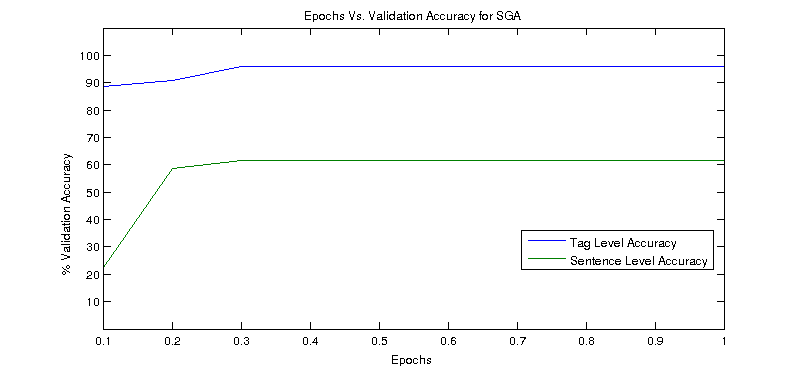
\includegraphics[width=\columnwidth]{EpochsVsValidationAccuracySGA}
\caption{Increse and saturation of validation accuracy with Epochs for SGA}
\label{fig:EpochsVsValidationAccuracySGA}
\end{figure}

%\caption{\label{tab:widgets}An example table.}
%\end{table}

\subsection{Collins Perceptron}

In this section, we present our results from training with the Collins Perceptron method and its subsequent performance upon the test data. As we have used multiple approaches, we refine the parameters for each of these approaches upon the validation set, and provide an independent statistic for the performance of each approach upon the test data. \textbf{The performance measures of different approaches upon the test data was not used in any way to make any choice regarding the model. However, once each approach had been refined upon the validation set, we evaluate the performance of the approach independently upon the test data to provide a comparitive analysis of the efficacy of each approach to the reader.}

\begin{itemize}

\item[(a)] Collins Perceptron with only POS features:\\

We train the model using only the 36 POS features. This approach allows us to explore the efficacy, or "worth", of the inherent part-of-speech of any word in determining the punctuation that follows it. We obtain the following results for different values of $\lambda$ upon the validation set.

\begin{center}
\begin{tabular}{|c|c|c|c|}
\hline
Epochs & $\lambda$ & Sentence Accuracy & Tag Accuracy\\\hline
1&	1	&	0.1961	&0.8346\\\hline
2&	0.1	&	0.1961	&0.8292\\\hline
1&	0.01&		0.1929	&0.8339\\\hline
1&	0.005&		0.1929	&0.8339\\\hline
1&	0.001	&	0.3632	&0.9085\\\hline
1&	0.0001&		0.1982	&0.8353\\\hline
\end{tabular}
\end{center}

Convergence is checked as defined in the previous section. For the optimal value of $\lambda$, we obtain peak accuracy as shown in Figure~\ref{fig:CP_oldFF}.

\begin{figure}[H]
\centering
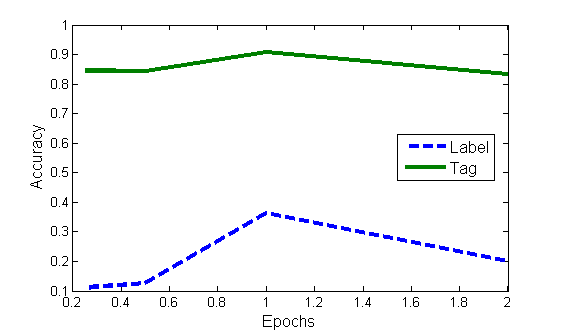
\includegraphics[width=\columnwidth]{CP_oldFF}
\caption{Collins Perceptron accuracy values with POS features.}
\label{fig:CP_oldFF}
\end{figure}

We use the optimal value of $\lambda = 0.001$ obtained to check the performance of the model upon the test set. We obtain the following results:

\begin{center}
\begin{tabular}{|c|c|c|c|}
\hline
Label Accuracy & Tag Accuracy\\\hline
0.2892	& 0.9125\\\hline
\end{tabular}
\end{center}

\item[(b)] Collins Perceptron with all features:\\

We train the model using the 36 POS features as well as the features that depend upon grammatical rules and positions of the words in a sentence. This approach allows us to explore the additional efficacy, or "worth", of these features in determining the punctuation that follows it. We obtain the following convergence plot using the same value of $\lambda$ and obtain peak accuracy upon the validation set as shown in Figure~\ref{fig:CP_newFF}.

\begin{figure}[H]
\centering
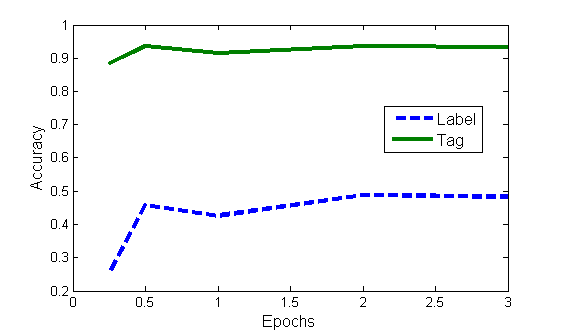
\includegraphics[width=\columnwidth]{CP_newFF}
\caption{Collins Perceptron accuracy values with all features.}
\label{fig:CP_newFF}
\end{figure}

We use this model to check the performance of the model upon the test set. We obtain the following results:

\begin{center}
\begin{tabular}{|c|c|c|c|}
\hline
Label Accuracy & Tag Accuracy\\\hline
0.4813	& 0.937\\\hline
\end{tabular}
\end{center}

\item[(c)] Collins Perceptron with all features with Regularization:

Through Grid Search, we obtain the following significant values for $\mu$ and $\lambda$ on the validation set.

\begin{center}
\begin{tabular}{|c|c|c|c|c|}
\hline
$Epochs$ & $\mu$ & $\lambda$ & Label Accuracy & Tag Accuracy\\\hline
1&	$10^{-7}$&	0.001&	0.258&	0.886\\\hline
1&	$10^{-6}$&	0.001&	0.311&	0.897\\\hline
1&	$10^{-5}$&	0.001&	0.309&	0.8944\\\hline
1&	$10^{-4}$&	0.0001&	0.325&	0.8947\\\hline
1&	$10^{-3}$&	0.00001&	0.247&	0.8771\\\hline
\end{tabular}
\end{center}


We obtain the following prediction performance upon the test set for the optimal value of $\mu = 10^{-4}$ and $\lambda = 0.325$ for only POS features, and all features.

\begin{center}
\begin{tabular}{|c|c|c|c|}
\hline
Features & Label Accuracy & Tag Accuracy\\\hline
POS Only & 0.2695	& 0.8983\\\hline
All & 0.2359 & 0.8856 \\\hline
\end{tabular}
\end{center}

It is interesting to note that the model with POS features only achieves a higher accuracy, with regularization, than the model trained with all features. \textbf{However, as we have chosen the model with all features based on our experiments on the validation set, we report the accuracy of the model with all features in the abstract of our report.}

\item[(d)] Running time of Collins Perceptron:

We also observe the running times of the Collins Perceptron training algorithm against the number of features, $J$. A typical graph is shown in Figure~\ref{fig:CP_run}.

\begin{figure}[H]
\centering
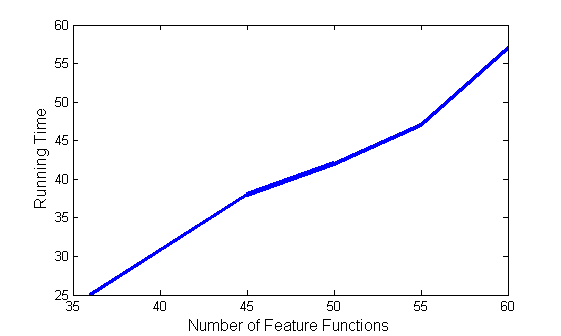
\includegraphics[width=\columnwidth]{CP_run}
\caption{Running time of Collins Perceptron against Number of Features.}
\label{fig:CP_run}
\end{figure}

\end{itemize}

\section{Findings and Lessons Learned}

From the results of our experiments and the observations in the above section, we attempt to draw some general conclusions about our model and the learning process.\\

1. One of the major bottlenecks in running experiments was the slow speed of training for SGA. We used a laptop running the latest generation Intel Haswell i5 processor and 4 GB of RAM. Initially, without any optimizations, SGA would take several hours to train on the entire training set. After applying the optimizations described in section 4.5, this running time was reduced to less than 2 hours. However, with many experiments to run, 2 hours was still a bit of a stretch and this required us to be very meticulous in ensuring a bug-free implementation.

2. Initially we used simple feature rules which only looked at individual POS tags in a specific position. However, we soon realized that the English language punctuation is too complex and we need a more nuanced approach. The feature functions based on basic grammar rules helped improve accuracy for such sentences. These feature functions have been described in detail in section 2.3.\\

3. CP runs faster than SGA in our code although they have similar time complexity. We found that this was because we could not use the fact that $A_a$ feature functions could be evaluated as $0$ for a given $i$ and $x$.Effectively, this made SGA slower for compuation of E and the Inference step. This led to a better performance of SGA.\\

4. Accuracy of SGA is greated than that of CP on a sentence level, however, tag level the accuracy is similar. We think this difference in accuracy is because CP is an approximtation of SGA.\\

5. As discussed in the notes\cite{classNotes}, the value of lambda did not change the accuracy of CP except for one value where it increased. We performed this experiment again to be sure but the result agreed. We later used this lambda for our experiments in CP.\\

6. We experienced a lot of issues with underflow while calculating weight vectors for SGA. Tuning both the learning rate($\lambda$) and strength of regularization($\mu$) was a rather cumbersome problem. A useful trick was to decrease $\lambda$ while decreasing $\mu$. Albeit,$\mu$ was decreased at a greater rate than  $\lambda$.\\

7. We found that low values of strength of regularization($\mu$) worked well. This is because, despite the low value, it still prevents the weights from becoming large enough for the model to overfit the data. If  regularization is not used at all, the model will perform worse on unseen data even if it is similar to training data. \\

8. We noticed that Stochastic Gradient Ascent did not converge for higher values of learning rate($\lambda$). We believe that this happens because the model relies more on information seen on recently processed sentences. It gains less information from previously seen sentences.\\

\bibliographystyle{abbrv}
\bibliography{Report}

\end{document}